\newif\ifsolutions
\solutionstrue % Show solutions
%\solutionsfalse % Hide solutions

\documentclass{article}
\usepackage{geometry}
\geometry{margin=1in}
\usepackage{tikz}
\usepackage{amssymb}

% fleqn allows setting indent of display math
\usepackage[fleqn]{amsmath}
\setlength{\mathindent}{0pt} % Set indent
% Disable equation numbering (https://tex.stackexchange.com/a/360378)
\makeatletter
\renewcommand\tagform@[1]{}
\makeatother

% Allow Unicode (some, e.g., © and £ at least)
% https://tex.stackexchange.com/questions/370278/is-there-any-reason-to-use-inputenc
\usepackage[utf8]{inputenc}

% Hyperlinks
\usepackage{hyperref}
\hypersetup{colorlinks=true, urlcolor=blue, linkcolor=blue}

% Prevent indentation of paragraphs
\setlength\parindent{0pt}
\setlength{\parskip}{\baselineskip}

% Spacing above/below equations
% https://tex.stackexchange.com/a/69678
\AtBeginDocument{%
 \abovedisplayskip=-\parskip
 \abovedisplayshortskip=-\parskip
 \belowdisplayskip=0pt
 \belowdisplayshortskip=0pt
}

% Allow 3 additional subsection levels
% https://tex.stackexchange.com/a/60212
\usepackage{titlesec}
\setcounter{secnumdepth}{6}
% H4 in HTML
\titleformat{\paragraph}{\normalfont\normalsize\bfseries}{\theparagraph}{1em}{}
\titlespacing*{\paragraph}{0pt}{3.25ex plus 1ex minus .2ex}{1.5ex plus .2ex}
% H5 in HTML
\titleformat{\subparagraph}{\normalfont\normalsize\bfseries}{\thesubparagraph}{1em}{}
\titlespacing*{\subparagraph}{0pt}{3.25ex plus 1ex minus .2ex}{1.5ex plus .2ex}
% H6 in HTML
\titleformat{\subsubparagraph}{\normalfont\normalsize\bfseries}{\thesubsubparagraph}{1em}{}
\titlespacing*{\subsubparagraph}{0pt}{3.25ex plus 1ex minus .2ex}{1.5ex plus .2ex}

% So enumerate at all levels is numbers
% https://tex.stackexchange.com/questions/78842/nested-enumeration-numbering
\renewcommand{\labelenumii}{\arabic{enumii}.}
\renewcommand{\labelenumiii}{\arabic{enumiii}.}
\renewcommand{\labelenumiv}{\arabic{enumiv}.}

\renewcommand{\mbox}{\text}
\newcommand{\ds}[0]{\displaystyle}
\newcommand{\ihat}[0]{\hat{\boldsymbol{\imath}}}
\newcommand{\jhat}[0]{\hat{\boldsymbol{\jmath}}}
\newcommand{\khat}[0]{\hat{\boldsymbol{k}}}
\newcommand{\xhat}[0]{\hat{\mathbf{x}}}
\newcommand{\yhat}[0]{\hat{\mathbf{y}}}
\newcommand{\zhat}[0]{\hat{\mathbf{z}}}
\newcommand{\rhat}[0]{\hat{\mathbf{r}}}
\newcommand{\bfvec}[1]{\vec{\mathbf{#1}}}
\newcommand{\bfcdot}[0]{\boldsymbol{\cdot}}

\usepackage{fancyhdr}
\pagestyle{fancy}
\lhead{Cross Products}
\rhead{\thepage}
\fancyfoot{}

\begin{document}

\section{Introduction}

The cross product of two vectors $\bfvec{v}$ and $\bfvec{B}$, written as $\bfvec{v}\times\bfvec{B}$, is a vector quantity with a magnitude of $|\bfvec{v}||\bfvec{B}|\sin\phi = vB\sin\phi$, where $\phi$ is the angle between the two vectors ($0 \le\phi \le 180^{\circ}$). The direction of $\bfvec{v}\times\bfvec{B}$ is perpendicular to the plane that contains both vectors. (There are two perpendicular directions, and the one to choose is determined using the cross--product right--hand rule; see your textbook for details.)

Three methods are commonly used for computing a cross--product. The first method (``By Inspection") is useful for certain simple problems, whereas the last two methods (``Multiply Through" and ``Determinant") apply to all problems. In principle, one can solve any problem knowing only the second or third methods. However, as the examples demonstrate, some methods lead to a solution with less effort than others. In addition, we recommend understanding all of the methods because it leads to insight into how cross--products work, and you are likely to encounter all of the methods in solutions that you read.

\section{The Circle Diagram}

Computing the cross--product of two vectors typically involves the cross-products of unit vectors. Unit vector cross products can be determined using the right--hand rule. However, some students find it easier to use a non--visual approach, which is described here. The possible cross products of unit vectors are

$$
\begin{align*}
\ihat\times\ihat & = \phantom{-}0 \qquad &
\jhat\times\jhat & = \phantom{-}0 \qquad &
\khat\times\khat & = \phantom{-}0 \qquad
\\
\ihat\times\jhat & =  \phantom{-}\khat &
\jhat\times\khat & = \phantom{-}\ihat  &
\khat\times\ihat & = \phantom{-}\jhat
\\
\jhat\times\ihat & = -\khat &
\khat\times\jhat & = -\ihat &
\ihat\times\khat & = -\jhat
\end{align*}
$$

There is a mnemonic (memory) device for remembering the second and third rows of this table.

\begin{itemize}

  \item If two unit vectors are crossed, the result is $\pm$, the unit vector not involved in the cross product.

  \item To determine the sign, connect the two crossed unit vectors by drawing the shortest line that connects the first to the second along the circle shown below.

  \item If the line drawn was clockwise, the cross product is positive. If the line drawn was negative, the cross product is negative.

\end{itemize}



\tikzset{every picture/.style={line width=0.75pt}} %set default line width to 0.75pt        

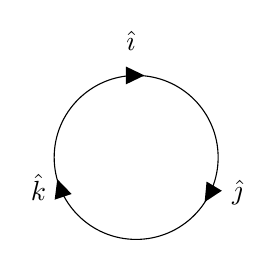
\begin{tikzpicture}[x=0.75pt,y=0.75pt,yscale=-1,xscale=1]
%uncomment if require: \path (0,119); %set diagram left start at 0, and has height of 119

%Shape: Circle [id:dp5988157550687865] 
\draw   (25.5,64.65) .. controls (25.5,42.83) and (43.18,25.15) .. (65,25.15) .. controls (86.82,25.15) and (104.5,42.83) .. (104.5,64.65) .. controls (104.5,86.47) and (86.82,104.15) .. (65,104.15) .. controls (43.18,104.15) and (25.5,86.47) .. (25.5,64.65) -- cycle ;
%Straight Lines [id:da42189417649788785] 
\draw    (29,81.14) -- (27.95,77.99) ;
\draw [shift={(27,75.14)}, rotate = 71.57] [fill={rgb, 255:red, 0; green, 0; blue, 0 }  ][line width=0.08]  [draw opacity=0] (8.93,-4.29) -- (0,0) -- (8.93,4.29) -- cycle    ;

%Straight Lines [id:da47415096212675123] 
\draw    (67,25.15) ;
\draw [shift={(69,25.15)}, rotate = 180] [fill={rgb, 255:red, 0; green, 0; blue, 0 }  ][line width=0.08]  [draw opacity=0] (8.93,-4.29) -- (0,0) -- (8.93,4.29) -- cycle    ;
%Straight Lines [id:da10747602373995879] 
\draw    (101,81.15) -- (99.54,83.57) ;
\draw [shift={(98,86.14)}, rotate = 300.99] [fill={rgb, 255:red, 0; green, 0; blue, 0 }  ][line width=0.08]  [draw opacity=0] (8.93,-4.29) -- (0,0) -- (8.93,4.29) -- cycle    ;


% Text Node
\draw (13,71.4) node [anchor=north west][inner sep=0.75pt]    {$\hat{k}$};
% Text Node
\draw (110,74.4) node [anchor=north west][inner sep=0.75pt]    {$\hat{\jmath }$};
% Text Node
\draw (59,2.4) node [anchor=north west][inner sep=0.75pt]    {$\hat{\imath }$};


\end{tikzpicture}


\subsection{Examples}

\begin{itemize}

  \item The cross product of $\jhat \times \khat$ requires drawing a clockwise line from $\jhat$ to $\khat$, so the result must be positive; the unit vector that was not a part of the cross--product is $\ihat$. Thus $\jhat \times \khat = \ihat$.

  \item The cross product of $\jhat \times \ihat$ requires drawing a counterclockwise line from $\jhat$ to $\ihat$, so the result must be negative; the unit vector that was not a part of the cross--product is $\khat$. Thus $\jhat \times \ihat = -\khat$.

\end{itemize}

\subsection{Problems}

Use the right--hand rule to determine the following cross--products. Then use the circle diagram to check your answer.

\ifsolutions
\textbf{Answer}:
A. $\khat \times \ihat = \boxed{\phantom{-}\jhat}\qquad$
B. $\khat \times \jhat = \boxed{-\ihat}\qquad$
C. $\ihat \times \khat = \boxed{-\jhat}$
\else
A. $\khat \times \ihat = \fbox{\phantom M}\qquad$
B. $\khat \times \jhat = \fbox{\phantom M}\qquad$
C. $\ihat \times \khat = \fbox{\phantom M}$
\fi

\section{By Inspection Method}

This method is most useful if the angle $\phi$ between the two vectors is given, obvious, or straightforward to compute. There are two possibilities.

\begin{enumerate}

  \item Both vectors point along different cartesian axis (so that $\phi=90^\circ$). In this case, the magnitude is the product of the vector lengths (which are positive by definition), and the direction is determined using the cross--product right--hand rule or the circle diagram.

        \textbf{Examples}:

    \begin{itemize}

      \item If $\bfvec{v}=2\ihat$ and $\bfvec{B}=3\jhat$, the cross product $\bfvec{v}\times\bfvec{B}=2\ihat\times3\jhat$ has a magnitude

            $|2\ihat||3\jhat|\sin 90^\circ = 6|\ihat||\jhat|\sin 90^\circ = 6$.

            The direction is $\khat$, which is determined using the right--hand rule on $\ihat\times\jhat$ or the circle diagram.

            Thus, $\bfvec{v}\times\bfvec{B} = 6\khat$

      \item If $\bfvec{v}=-2\jhat$ and $\bfvec{B}=3\khat$, the cross product $-2\jhat\times3\khat$ has a magnitude

            $|-2\jhat||3\khat|\sin 90^\circ = 2\cdot 3|\jhat||\khat|\sin 90^\circ = 6$.

            The direction is $-\ihat$, which is determined using the right--hand rule on $-\jhat\times\khat$ or the circle diagram.

            Thus, $\bfvec{v}\times\bfvec{B}=-6\ihat$

    \end{itemize}

  \item Both vectors lie in the same coordinate plane (e.g., one of $x$--$y$, $x$--$z$, or $y$--$z$). In this case, compute the magnitude using $|\bfvec{v}||\bfvec{B}|\sin\phi$ and the direction using the cross--product right--hand rule.

        \textbf{Examples}:

      \begin{itemize}

        \item If $\bfvec{v}=\ihat$ and $\bfvec{B}=\ihat$, the cross product $\bfvec{v}\times\bfvec{B}=\ihat\times\ihat$ is zero because its magnitude is $|\ihat||\ihat|\sin 0 = 1\cdot 1 \cdot 0$.

        \item If $\bfvec{v}=\ihat$ and $\bfvec{B}=\ihat+\jhat$, the cross product $\bfvec{v}\times\bfvec{B}= \ihat\times(\ihat+\jhat)$ has a magnitude of $|\ihat||\ihat+\jhat|\sin 45^\circ = 1\cdot \sqrt{2} \sin 45^\circ = 1$

              (From a diagram, it should be straightforward to see that the angle between $\ihat$ and $\ihat+\jhat$ is $45^\circ$ and the magnitude of $\bfvec{B}$ is $\sqrt{2}$).

              The direction is $\khat$, which can be determined using the cross--product right--hand rule. Thus, $\bfvec{v}\times\bfvec{B}=\sqrt{2} \sin 45^\circ\khat = \khat$.

      \end{itemize}

\end{enumerate}

\ifsolutions

\else

\newpage
\fi

\subsection{Problems}

Compute $\bfvec{v}\times\bfvec{B}$ for each of the following cases.

\ifsolutions
\textbf{Answers}:

    \begin{itemize}

      \item $\bfvec{v}=v_x\ihat\quad$ and $\quad\bfvec{B}=\phantom{-}B_y\jhat$, $\quad\bfvec{v}\times\bfvec{B} = \boxed{v_xB_y\khat}$

      \item $\bfvec{v}=v_x\ihat\quad$ and $\quad\bfvec{B}=-B_y\jhat$, $\quad\bfvec{v}\times\bfvec{B} = \boxed{-v_xB_y\khat}$

      \item $\bfvec{v}=v_z\khat\quad$ and $\quad\bfvec{B}=\phantom{-}B_y\jhat$, $\quad\bfvec{v}\times\bfvec{B} = \boxed{-v_zB_y\ihat}$

    \end{itemize}
\else
\vskip 60pt

    \begin{itemize}

      \item $\bfvec{v}=v_x\ihat\quad$ and $\quad\bfvec{B}=\phantom{-}B_y\jhat$, $\quad\bfvec{v}\times\bfvec{B} = \fbox{\qquad\phantom M}$

    \end{itemize}

\vskip 60pt

    \begin{itemize}

      \item $\bfvec{v}=v_x\ihat\quad$ and $\quad\bfvec{B}=-B_y\jhat$, $\quad\bfvec{v}\times\bfvec{B} = \fbox{\qquad\phantom M}$

    \end{itemize}

\vskip 60pt

    \begin{itemize}

      \item $\bfvec{v}=v_z\khat\quad$ and $\quad\bfvec{B}=\phantom{-}B_y\jhat$, $\quad\bfvec{v}\times\bfvec{B} = \fbox{\qquad\phantom M}$

    \end{itemize}
\fi

\vskip 36pt

\vskip 0.75pt

Compute $\bfvec{v}\times\bfvec{B}$ based on the information in the following diagrams. Write your answers below each diagram.

\input{figures/Diagram_I.tikz?1711468265551}

\ifsolutions
\textbf{a.}
$|\bfvec{v}\times\bfvec{B}| = |\bfvec{v}||\bfvec{B}|\sin 30^\circ = 60\sin 30^\circ$. From the right--hand rule, the direction is $-\khat$. So $\bfvec{v}\times\bfvec{B}=-60\sin 30^\circ\khat$

\textbf{b.} Here we are not given the angle, but it can be computed from $\sin\phi=6/\sqrt{6^2+7^2}$. In addition, we need to compute $|\bfvec{B}|$, which is $\sqrt{6^2+7^2}$. So $|\bfvec{v}\times\bfvec{B}| = |\bfvec{v}||\bfvec{B}|\sin\phi = 42$. The direction is $-\ihat$, so $\bfvec{v}\times\bfvec{B}=-42\ihat$. Note that because we were given vector components and not the angle between the vectors, several steps were needed for this method. A fast approach for this problem is to use the ``Multiply Through" method, covered in the next section.
\else

\newpage
\fi

\section{Multiply Through Method}

This method is most useful when each of the vectors in the cross--product has two or fewer components. Otherwise, the Determinant Method, covered in the next section, is preferred.

Write the vectors in component form and then ``multiply through" in a way that is similar to ``multiplying through" to convert the product of sums into a sum of products. For example,

$$(a)\cdot(b+c) = (a\cdot b) + (a\cdot c)$$

but replace the multiplication symbol ($\cdot$) with the cross product symbol ($\times$). Note that order matters -- although with regular multiplication we can also write $a(b+c) = (b\cdot c) + (c\cdot d)$, when using this method, the first parentheses on the left--hand side must appear first in the mulitplications on the right--hand side.

Another example is the first--outer--inner--last (foil) case:

$$(a+b)(c+d)=(a\cdot c) + (a\cdot d) + (b\cdot c) + (b\cdot d)$$

\subsection{Examples}

\begin{itemize}

  \item If $\bfvec{v}=v_x\ihat$ and $\bfvec{B}=B_x\ihat+B_y\jhat$, then

        $$
        \begin{align*}
        \bfvec{v}\times\bfvec{B} &= v_x\ihat\times(B_x\ihat+B_y\jhat)\\
        &= v_xB_x(\ihat\times\ihat) + v_xB_y(\ihat\times\jhat)\\
        &= 0 + v_xB_y\khat\\
        &= v_xB_y\khat
        \end{align*}
        $$

  \item If $\bfvec{v}=v_x\ihat$ and $\bfvec{B}=B_x\ihat+B_y\jhat + B_z\khat$, then

        $$
        \begin{align*}
        \bfvec{v}\times\bfvec{B} &= v_x\ihat\times(B_x\ihat+B_y\jhat+B_z\khat) \\
        & = v_xB_x(\ihat\times\ihat) + v_xB_y(\ihat\times\jhat) + v_xB_z(\ihat\times\khat)\\
        & = 0 + v_xB_y\khat - v_xB_z\jhat
        \end{align*}
        $$

\end{itemize}

\ifsolutions

\else

\newpage
\fi

\subsection{Problems}

Use the ``Multiply Through" method for these problems.

Compute $\bfvec{v}\times\bfvec{B}$ and write your answer after the equal sign for each of the following cases.

\ifsolutions
    \begin{itemize}

      \item $\bfvec{v}=v_x\ihat+v_y\jhat+v_z\khat\quad$ and $\quad\bfvec{B}=B_x\ihat$, $\quad\bfvec{v}\times\bfvec{B} = \boxed{-v_yB_x\ihat+v_zB_x\jhat}$

    \end{itemize}
\else
\vskip 48pt

    \begin{itemize}

      \item $\bfvec{v}=v_x\ihat+v_y\jhat+v_z\khat\quad$ and $\quad\bfvec{B}=B_x\ihat$, $\quad\bfvec{v}\times\bfvec{B} = \fbox{\qquad\qquad\qquad\phantom M}$

    \end{itemize}
\fi

\ifsolutions
    \begin{itemize}

      \item $\bfvec{v}=v_x\ihat+v_y\jhat\quad$ and $\quad\bfvec{B}=B_x\ihat+B_y\jhat$, $\quad\bfvec{v}\times\bfvec{B} = \boxed{(v_xB_y-v_yB_x)\khat}$

    \end{itemize}
\else
\vskip 48pt

    \begin{itemize}

      \item $\bfvec{v}=v_x\ihat+v_y\jhat\quad$ and $\quad\bfvec{B}=B_x\ihat+B_y\jhat$, $\quad\bfvec{v}\times\bfvec{B} = \fbox{\qquad\qquad\qquad\phantom M}$

    \end{itemize}
\fi

\vskip 0.75pt

Compute $\bfvec{v}\times\bfvec{B}$ based on the information in the following diagrams by writing $\bfvec{v}$ and $\bfvec{B}$ in vector notation and using the Multiply Through Method. Show your work in the space below each diagram.

\input{figures/Diagram_II.tikz}

\ifsolutions
\textbf{a.}

$\bfvec{v}=10\cos 45^\circ\ihat + 10\sin 45^\circ\jhat$

$\quad\bfvec{B}=6\cos 15^\circ\ihat + 6\sin 15^\circ\jhat$

$$
\begin{align*}
\quad\bfvec{v}\times\bfvec{B} &= (10\cos 45^\circ \cdot 6\sin 15^\circ-10\sin 45^\circ \cdot 6\cos 15^\circ)\khat\\\\
&= 60\sin 30^\circ\khat
\end{align*}
$$

where the last equality follows from a trig identity. Note that this problem is much more easily solved using the ``By Inspection" method covered in the previous section.

\textbf{b.}

$$
\begin{align*}
\bfvec{v}\times\bfvec{B} &= 7\khat \times (6\jhat + 7\khat) \\\\
&= 42(\khat\times\jhat + \khat\times\khat) \\\\
&= -42\ihat
\end{align*}
$$

Note that the result is the same as if we crossed only the $y$--component of $\bfvec{B}$ with $\bfvec{v}$. The reason is that we can re--write the cross product $\bfvec{v}\times\bfvec{B}$ as

$\bfvec{v}\times\bfvec{B} = \bfvec{v}\times\bfvec{B}_\parallel+\bfvec{v}\times\bfvec{B}_\perp$

where the parallel and perpendicular are with respect to $\bfvec{v}$. The term $\bfvec{v}\times\bfvec{B}_\parallel$ is always zero, so another form of $\bfvec{v}\times\bfvec{B}$ that is sometimes used is when it is straightforward to determine $\bfvec{B}_\perp$ is

$\bfvec{v}\times\bfvec{B} = \bfvec{v}\times\bfvec{B}_\perp$

In this problem, we can read off from the diagram $\bfvec{B}_\perp=6\jhat$, so 

$\bfvec{v}\times\bfvec{B} = \bfvec{v}\times\bfvec{B}_\perp = 7\khat\times 6\jhat = -42\ihat$

\textbf{c.}

$\bfvec{B}=6\khat$

and

$\bfvec{v}=3\cos 45^\circ\ihat + 3\sin 45^\circ\jhat = \ds \frac{3}{\sqrt{2}}(\ihat+\jhat)$, so

$$
  \begin{align*}
   \bfvec{v}\times\bfvec{B} & = \frac{3}{\sqrt{2}}(\ihat+\jhat)\times 6\khat \\\\
   & = \frac{18}{\sqrt{2}}(\ihat\times\khat + \jhat\times\khat) \\\\
   & = \frac{18}{\sqrt{2}}(\ihat - \jhat)
  \end{align*}
  $$
\else

\newpage
\fi

\section{Determinant Method}

To find all non--zero terms that would have resulted using the Determinant Method, write the cross product in matrix determinant form as follows and compute its determinant. (This requires that you have memorized the procedure for computing the determinant of a $3\times 3$ matrix.) The most general problem and steps are as follows.

$$
\begin{align*}
\bfvec{v}\times\bfvec{B}
&=
\begin{vmatrix}
\ihat&\jhat&\khat\\
v_x&v_y&v_z\\
B_x&B_y&B_z\\
\end{vmatrix}
\\\\ &=
\begin{vmatrix}
v_y & v_z \\
B_y & B_z 
\end{vmatrix} \ihat - \begin{vmatrix}
v_x & v_z \\
B_x & B_z 
\end{vmatrix} \jhat +  \begin{vmatrix}
v_x & v_y \\
B_x & B_y 
\end{vmatrix} \khat
\\\\ &=
(v_yB_z - v_zB_y)\ihat -(v_xB_z - v_zB_x)\jhat +(v_xB_y - v_yB_x)\khat
\end{align*}
$$

\subsection{Example}

If $\bfvec{v}=2\ihat$ and $\bfvec{B}=3\ihat+4\jhat$, then

$$
\begin{align*}
\bfvec{v}\times\bfvec{B}
&=
\begin{vmatrix}
\ihat&\jhat&\khat\\
2&0&0\\
3&4&0\\
\end{vmatrix}
\\\\ &=
\begin{vmatrix}
0 & 0 \\
4 & 0 
\end{vmatrix} \ihat - \begin{vmatrix}
2 & 0 \\
3 & 0 
\end{vmatrix} \jhat +  \begin{vmatrix}
2 & 0 \\
3 & 4 
\end{vmatrix} \khat
\\\\ &=
0\ihat - 0\jhat + 8\khat
\end{align*}
$$

(One could have used the general formula given above, but here we assume you don't have it memorized.)

\subsection{Problem}

If $\bfvec{v}=1\ihat+2\jhat$ and $\bfvec{B}=3\ihat+4\jhat$, use the Determinant Method to find $\bfvec{v}\times\bfvec{B}$. Show your work.

\ifsolutions
$$
\begin{align*}
\bfvec{v}\times\bfvec{B}
&=
\begin{vmatrix}
\ihat&\jhat&\khat\\\\
1&2&0\\\\
3&4&0\\\\
\end{vmatrix}
\\\\ &=
\begin{vmatrix}
2 & 0 \\\\
4 & 0 
\end{vmatrix} \ihat - \begin{vmatrix}
1 & 0 \\\\
3 & 0 
\end{vmatrix} \jhat +  \begin{vmatrix}
1 & 2 \\\\
3 & 4 
\end{vmatrix} \khat
\\\\ &=
0\ihat - 0\jhat + (4-6)\khat
\\\\ &=
-2\khat
\end{align*}
$$
\fi

\end{document}